% Horizon penetrating coordinates (vs. Schwarzschild coordinates)
% for a black hole spacetime, with excision
% Author: Jonah Miller
\documentclass[tikz,border=0pt]{standalone}
\usepackage{tikz}
\usetikzlibrary{arrows}
\usetikzlibrary{arrows.meta}
\usetikzlibrary{decorations.markings}
\usepackage{pgfplots}
\usepackage{amsmath}
\usetikzlibrary{decorations.pathreplacing}

\usepgfplotslibrary{fillbetween}

%\tikzset{>={Latex[length=3mm]}}

\tikzstyle{mybox} = [draw=black,
    rectangle, inner sep=10pt, inner ysep=10pt]
\tikzstyle{fancytitle} =[fill=blue!30, text=black]

\begin{document}
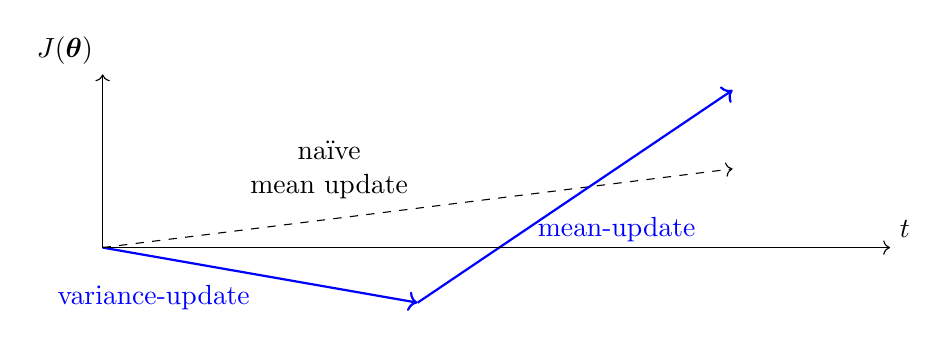
\begin{tikzpicture}[xscale=2]

\draw[->,black,dashed] (0,0) -- (4,1) node[midway,above left]{\begin{minipage}{2cm}\centering na\"ive \\ mean update\end{minipage}} ;%node[right,black]{$J(\boldsymbol{\theta}')$};
\draw[->, thick, blue] (0,0) -> (2,-0.7) node[midway,below left]{variance-update};
\draw[->, thick, blue] (2,-0.7) -- (4,2) node[midway,xshift=15pt,yshift=-12pt]{mean-update};% node[right,black]{$J(\boldsymbol{\theta}')$};

\draw[->] (0,0) -- (5,0) node[above right]{$t$};
\draw[->] (0,0) -- (0,2.2) node[above left]{$J(\boldsymbol{\theta})$};
%\draw [decorate,decoration={brace,amplitude=5pt,mirror,raise=0pt},xshift=0,yshift=0pt]
%(4.1,0) -- (4.1,1) node [black,midway,xshift=35pt,text width=1.5cm] 
%{\footnotesize greedy update};

%\draw[dashed] (4,2) -- (5.5,2);

%\draw [decorate,decoration={brace,amplitude=5pt,mirror,raise=0pt},xshift=0,yshift=0pt]
%(5.5,0) -- (5.5,2) node [black,midway,xshift=35pt,text width=1.2cm] 
%{\footnotesize smart update};

%\node[right,yshift=10pt] at (4,2) {\begin{minipage}{4cm} $$  \begin{cases} w \gets w + \beta \nabla_w \mathcal{L}(\boldsymbol{\theta}) \\ \boldsymbol{v} \gets \boldsymbol{v} + \alpha \nabla_{\boldsymbol{v}}J(\boldsymbol{\theta}) \end{cases} $$ \end{minipage}};

%\node[right,xshift=5pt] at (4,1) {$\boldsymbol{v} \gets \boldsymbol{v} + \alpha \nabla_{\boldsymbol{v}}J(\boldsymbol{\theta})$};


\end{tikzpicture}
\end{document}